% Figure: --mem-fraction-static x --cuda-graph-max-bs vs total throughput.
% Data: NUMBERS.md (ground truth), verified against
%   firmus/optimisation/simple/memfrac_logs/{regular,512,724}_batch/memfrac_0.9*.log
% System B (Firmus H200), 2 nodes x 8 GPU, TP=16, Singularity container,
% sglang.bench_offline_throughput, DeepSeek-R1, 2000 ShareGPT prompts.
% bs=724 OOMs at 0.93; everything OOMs at 0.94.
%
% Standalone: pdflatex memfrac_tuning_pgf.tex
% For the paper: copy the tikzpicture into main.tex (needs \usepackage{pgfplots},
% \pgfplotsset{compat=1.17}) — width is already \columnwidth-friendly.
\documentclass[border=2pt]{standalone}
\usepackage{pgfplots}
\pgfplotsset{compat=1.17}
\newlength{\figwidth}\setlength{\figwidth}{8.45cm}% ACM \columnwidth; in the paper use \columnwidth

\definecolor{bsA}{HTML}{999999}% 256
\definecolor{bsB}{HTML}{E69F00}% 512
\definecolor{bsC}{HTML}{0072B2}% 724
\definecolor{oomred}{HTML}{D55E00}

\begin{document}
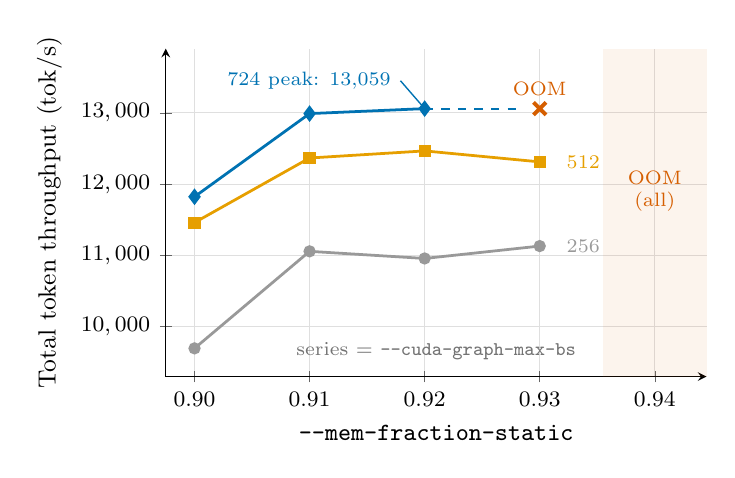
\begin{tikzpicture}
\begin{axis}[
    width=\figwidth, height=0.68\figwidth,
    xlabel={\texttt{--mem-fraction-static}},
    ylabel={Total token throughput (tok/s)},
    xmin=0.8975, xmax=0.9445,
    ymin=9300, ymax=13900,
    xtick={0.90,0.91,0.92,0.93,0.94},
    x tick label style={/pgf/number format/.cd, fixed, fixed zerofill, precision=2},
    scaled y ticks=false,
    y tick label style={/pgf/number format/.cd, fixed, use comma=false, 1000 sep={,}},
    ytick={10000,11000,12000,13000},
    axis lines=left,
    clip=false,
    grid=both, grid style={gray!25, line width=0.3pt},
    tick style={black!60},
    label style={font=\small},
    tick label style={font=\footnotesize},
]

% ---- OOM band at 0.94 (all series) ----
\addplot[draw=none, fill=oomred, fill opacity=0.07, forget plot]
    coordinates {(0.9355,9300) (0.9445,9300) (0.9445,13900) (0.9355,13900)} -- cycle;

% ---- cuda-graph-max-bs = 256 ----
\addplot[color=bsA, mark=*, mark size=1.7pt, line width=1.0pt]
    coordinates {(0.90,9695.82) (0.91,11057.12) (0.92,10957.14) (0.93,11130.89)};

% ---- cuda-graph-max-bs = 512 ----
\addplot[color=bsB, mark=square*, mark size=1.7pt, line width=1.0pt]
    coordinates {(0.90,11460.25) (0.91,12366.44) (0.92,12465.98) (0.93,12311.90)};

% ---- cuda-graph-max-bs = 724 ----
\addplot[color=bsC, mark=diamond*, mark size=2.2pt, line width=1.0pt]
    coordinates {(0.90,11822.57) (0.91,12989.38) (0.92,13059.21)};

% ---- direct series labels (right of last point) ----
\node[font=\scriptsize, color=bsA, anchor=west] at (axis cs:0.9315,11130.89) {256};
\node[font=\scriptsize, color=bsB, anchor=west] at (axis cs:0.9315,12311.90) {512};
\node[font=\scriptsize, color=black!55, anchor=south]
    at (rel axis cs:0.5,0.02) {series = \texttt{--cuda-graph-max-bs}};

% ---- OOM markers ----
% bs=724 OOMs at 0.93: dashed continuation from last good point to a red x
\draw[bsC, dashed, line width=0.8pt]
    (axis cs:0.92,13059.21) -- (axis cs:0.9285,13059.21);
\addplot[only marks, mark=x, mark size=3.2pt, color=oomred,
         mark options={line width=1.4pt}, forget plot]
    coordinates {(0.93,13059.21)};
\node[font=\scriptsize, color=oomred] at (axis cs:0.93,13330) {OOM};
% 0.94: OOM for every configuration
\node[font=\scriptsize, color=oomred, align=center] at (axis cs:0.94,11900) {OOM\\(all)};

% ---- peak annotation ----
\node[font=\scriptsize, color=bsC, anchor=west] (pk) at (axis cs:0.902,13450) {724 peak: 13,059};
\draw[bsC, line width=0.5pt] (pk.east) -- (axis cs:0.92,13059.21);

\end{axis}
\end{tikzpicture}
\end{document}
